%\documentclass[USenglish,pdftex,compress,10pt,svgnamesi,handout]{beamer}
\documentclass[USenglish,pdftex,compress,10pt,svgnamesi]{beamer}%


\usepackage{tikz}
\usetikzlibrary{positioning}
\usetikzlibrary{bayesnet}

\usefonttheme[onlymath]{serif}
\usepackage[ansinew]{inputenc}      % direkte Eingabe von Umlauten
\usepackage{graphicx}   % picture inclusion
\usepackage{amsmath}    % extended math stuff
\usepackage{amsfonts}   % corresponding fonts
\usepackage{bm}         % improved Greek bold math

\usepackage[english]{babel}

\usepackage[square]{natbib}  % reference 
\usepackage{booktabs}
\usepackage{ae}          % PDF-compatible fonts

\setbeamertemplate{footline}[frame number]

\newcommand{\imgcrop}[4]{  % filename, title, boxwidth, viewport
\centering\begin{beamerboxesrounded}[upper=fig,lower=block body,width=#3,shadow=true]{#2}
\includegraphics[width=\textwidth,viewport=#4]{pics/#1}
\end{beamerboxesrounded}
}
\newcommand{\imgbox}[3]{   % filename, title, boxwidth
\centering\begin{beamerboxesrounded}[upper=fig,lower=block body,width=#3,shadow=true]{#2}
\includegraphics[width=\textwidth]{pics/#1}
\end{beamerboxesrounded}
}

\newenvironment{poll}
{\begin{frame}<handout:0>
\frametitle{poll}
	\color[rgb]{0,.3,0}}
{\end{frame}}


\usetheme{Boadilla}
\usecolortheme[rgb={0,0.4,0}]{structure}
  \setbeamertemplate{enumerate items}[square]
  \setbeamertemplate{itemize items}[square]

\author{Patrick van der Smagt}
\hypersetup{%
	pdfauthor={Patrick van der Smagt}%
}


\def\target{z}


%\newcommand{\be}{\begin{equation}}
%\newcommand{\bel}[1]{\begin{equation}\label{#1}}
%\newcommand{\ee}{\end{equation}}
\newcommand*\abs[1]{\left\lvert#1\right\rvert}      % absolute value
\newcommand*\avg[1]{\left<#1\right>}                % average
\newcommand*\C{\mathcal{C}}                         % class C (for classification)

\let\orid=\d %for lower dot accent use \orid now
\renewcommand*\d[3][]{                              % differetial quotient
  \def\next{#1}%
  \ifx\empty\next
    \frac{\text{d}#2}{\text{d} #3}
  \else
    \frac{{\text{d}#2}^{#1}}{\text{d}^{#1} #3}
  \fi}
\newcommand*\D[3][]{                                % partial derivative
  \def\next{#1}%
  \ifx\empty\next
    \frac{\partial#2}{\partial #3}
  \else
    \frac{{\partial#2}^{#1}}{\partial^{#1} #3}
  \fi}
\newcommand{\Def}[1]{\alert{#1}}                    % first occurrence of a new term
\newcommand{\Annot}[1]{\qquad\text{#1}}             % annotation in (short) equation
\newcommand{\Set}[1]{\mathcal{#1}}                  % mathematical set
\newcommand*\Det[1]{\left\lvert#1\right\rvert}      % determinant
\newcommand*\diff{\text{d}}                         % differential
\newcommand*\DX{\,\text{d}x}                         % differential dx
\newcommand*\DY{\,\text{d}y}                         % differential dy
\newcommand*\E{\mathbb{E}}  % expectation value
\renewcommand*\H{\mathrm{H}}                          % Entropy
\newcommand*\KL{\mathrm{KL}}                        % Kullback-Leibler divergence
\newcommand\imagi{\text{i}}                         % \sqrt{-1} == \imagi (imaginary)
\newcommand*\Mtx[1]{\bm{{#1}}}                      % matrix quantity
\newcommand{\Norm}[1]{\lVert#1\rVert}               % norm of a matrix or vector
\newcommand*\N{\mathcal{N}}                         % Normal distribution
\newcommand*\Nset{\mathbb{N}}                       % set of natural numbers
\newcommand\Order[1]{\mathcal{O}(#1)}               % order operator
\newcommand\nate{\text{e}}                          % base of ln == \exp (natural e)
\newcommand*\Operator[1]{\mathcal{#1}}              % operator quantity
\newcommand{\ParBeg}[1]{\structure{#1}}             % new paragraph, similar to description
\newcommand*\Q{\mathbb{Q}}                          % set Q {rational numbers}
\newcommand*\R{\mathbb{R}}                          % set R {real numbers}
\newcommand*\T{^{\text{T}}}                         % transpose
\newcommand*\Tensor[1]{\bm{\mathsf{#1}}}            % tensor quantity
\newcommand{\var}{\text{var}}
\renewcommand*\Vec[1]{\bm{{#1}}}                    % vector quantity

\newcommand*\Z{\mathbb{Z}}                          % set Z {... -1, 0, 1, ...}

\newcommand{\mub}{\Vec{\mu}}
\DeclareMathOperator*{\argmax}{arg\,max}
\DeclareMathOperator*{\argmin}{arg\,min}
\newcommand*\F{\mathcal{F}}
\newcommand{\ra}[1]{\renewcommand{\arraystretch}{#1}}

\newcommand\keyword[1]{\textbf{$\rightarrow$ #1}}



\def\function{f}
\def\model{\hat\function}


\graphicspath{{pics/}}
\usepackage{picinpar}

\parskip2ex

\def\Vec#1{\textbf{#1}}
\def\bfx{{\Vec x}}
\def\bfw{{\Vec w}}
\def\cl#1{{\cal #1}}
\newcommand{\scalar}[2]{#1^T#2}
\newcommand{\scalarold}[2]{\left<#1,#2\right>}



% =====================================================================
% Titel etc.
\hypersetup{pdftitle={Introduction}}

\title{Introduction}
\date{March 2023}
% =====================================================================
\begin{document}

%'''''''''''''''''''''''''''''''''''''''''''''''''''''''''
\begin{frame}
	\titlepage
\end{frame}


\begin{frame}
You have data from a stochastic system:
\begin{itemize}
  \item from an airport camera,
  \item from a camera seeing an insect flying, a body suit on a human, \dots
  \item weather observations, stock market data,
  \item a tactile sensor on a robot hand, etc.
\end{itemize}
and you want to use these data to
\begin{itemize}
  \item detect suspicious behaviour,
  \item classify movement,
  \item predict future data,
  \item control a system
\end{itemize}
How?

%\frametitle{1st generation machine intelligence:  expert systems (1960--1980s)}
%\begin{flushright}{    \it
%An expert system is a computer system that emulates, or acts in all respects, with the decision-making capabilities of a human expert.}
%\\ \medskip
% Edward Feigenbaum, Stanford University
%\end{flushright}
%
%
%\begin{itemize}
%\item major components: knowledge base, inference engine, and user interface
%\item knowledge is encoded as IF . . . THEN rules
%\end{itemize}
%Problem: 
%\begin{itemize}
%\item combinatorial explosion of rules
%\item rules are made by hand from human experts
%\item suffer from the the challenge of uncertainty
%\end{itemize}
%---it does not generalise.
\end{frame}






\begin{frame}
The description is simple, in the form a model of your stochastic process:
$$
y = \function(x)
$$
where $y$, $x$ are vectors, and $\function()$ is the underlying model.

Consider the above also in the special form
$$
x_{t+1} = \function (x_t)
$$
where we use the Markov assumption.

Key question: how do we get $f()$?
%\frametitle{2nd generation machine intelligence: neural networks (1980s--1990s)}
%\begin{itemize}
%\item learn from data only
%\item can (theoretically) represent any kind of data
%\end{itemize}
\end{frame}



\begin{frame}
\frametitle{approximating $\function()$ through system knowledge}
If, e,g., we find all red objects in HSV space\\
 -- or we compute the Cartesian end position of a robot arm by inverse kinematics\\
 -- or we compute radiation of an exploding supernova\\
 -- or we want to determine a plant by analysing stem, leaves, flowers\\
 --\\
in each of these cases, we formalise expert knowledge in terms of a set of rules or decisions.

This is known classical control, expert systems, etc.

It is your best solution if your approximation (`model') $\model_\theta()$ to $\function()$ can be described at your desired accuracy.
The description of $\model()$ is obtained using innate knowledge of $\function$.
How do you know if your accuracy is good enough?
\end{frame}

\begin{frame}
\frametitle{approximating $f()$ when system knowledge fails}
If, e.g., you want to recognise faces, or a plant from a picture\\
 -- or want to create a programme to play go\\
 -- or want to find good grip positions on a random object\\
 -- or want to recognise a composer by listening to their music\\
 --\\
in each of these cases, the number of cases is too large to exhaustively describe accurately enough.

We have no detailed knowledge of $\function()$, and instead we use a general form for $\model()$ that can represent any function.
\end{frame}
\begin{frame}
But both approaches are in principle the same:
\begin{enumerate}
\item[1.] create a parameterised model $\model(x,\theta)$
\item[2.] find best values for the parameters $\theta$
\end{enumerate}

How do we do the second step?  Two options:\\
\begin{enumerate}
\item[a.] we make $\model$ behave as close as possible to $\function$ \\(e.g., maximise number of go games won)
\item[b.] we make $\model$ be as close as possible to $\function$ through
$
\min_\theta | \model_\theta(x) - \function(x) |.
$

Failing $\function$, we sample $\function$ in $\{x_i, y_i\}$ to 
$
\min_\theta \sum_i | \model_\theta(x_i) - y_i |
$
as a proxy.

We can write this as $\max_\theta \prod_i p_\theta (y_i \mid x_i)$.
\end{enumerate}

\end{frame}

\begin{frame}

The basic problem that we study in probability theory:
\begin{center}
Given a data generating process,\\ what are the properties of the outcomes?
\end{center}
The basic problem of statistics (or better statistical inference) \\is the inverse of probability theory:
\begin{center}
Given the outcomes,\\
what can we say about the process that generated the data?
\end{center}
Statistics uses the formal language of probability theory.

\end{frame}



\begin{frame}
\frametitle{discriminative vs.\ generative models}

The above describes \textit{discriminative} models, which map inputs to outputs and are described by $p(y|x)$.

Often we are interested in \textit{generative} models, represented by \\
$p(x, y)$ (if we have labels) or \\
$p(x)$ (if we have no labels). 


We can still measure quality, through $\max_\theta \prod_i p_\theta (x_i)$.

Generative models can be used to generate new data, or to test the likelihood of a datum.

\end{frame}



\begin{frame}
\frametitle{examples of discriminative models}

This is nothing new. Typically, such models use
$$\model_\theta(x) = \sum_k \theta_k s_k (x)$$
which describes, for instance, Fourier transform, polynomials, etc.

This general form is known as \textit{linear regression}, because the regression function is linear in the parameters $\theta$.

This is important as we have a closed-form solution to find $\theta$.

In the connectionism paradigm, the models can be drawn like this:

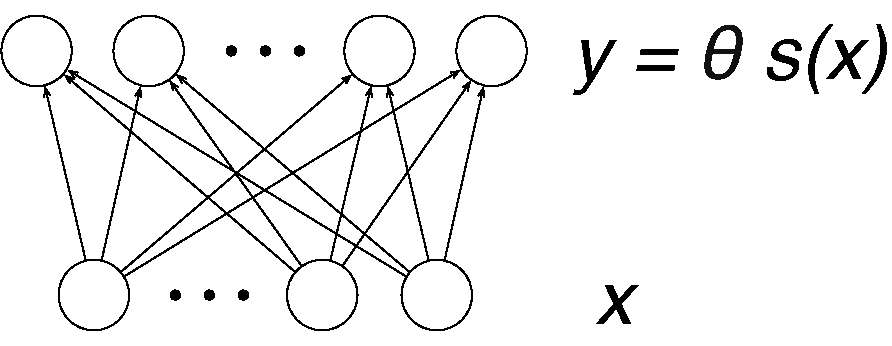
\includegraphics[scale=0.3]{nn0.pdf}
aka the perceptron
\end{frame}

\begin{frame}
\frametitle{curse of dimensionality}

Even if $x$ is only 100-dimensional

and you have a trillion data, 

\quad those data cover only $10^{-18}$ of the input space.\\[3ex]

This can be very problematic for such models.  

We need models that generalise further.
\end{frame}

\begin{frame}
\frametitle{extending the connectionist idea}
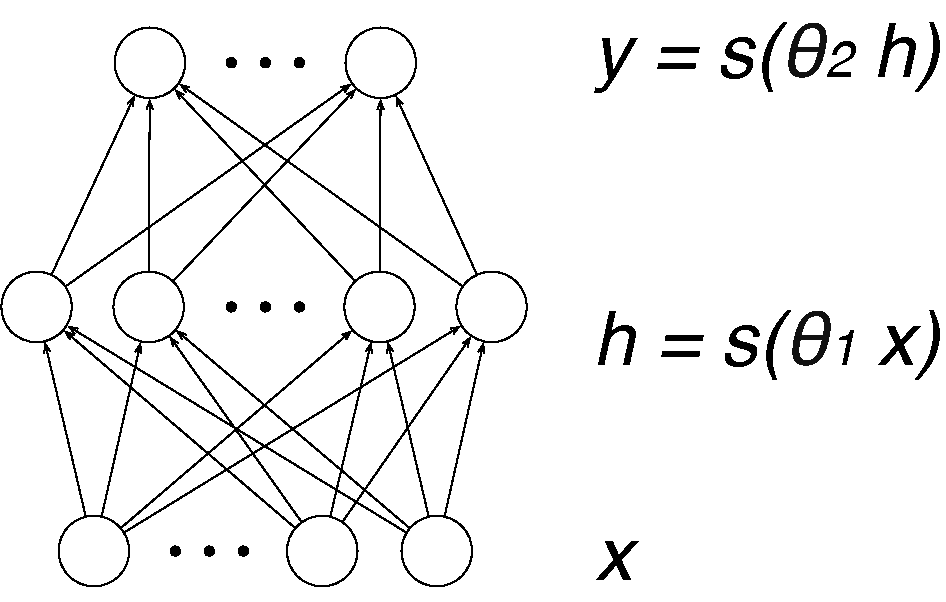
\includegraphics[scale=0.3]{nn1.pdf}
\qquad{\tiny did you see the small trick I did?}

That's a great idea from the 1970s which suggests,
$$\model_\theta(x) = \sum_k \theta_k s \left(\sum_i \theta_l x\right)$$
and the neural network (= multi-layer perceptron) is born.

Problem: finding $\theta$ can no longer be done closed-form.\\
Gradient-based optimisation is the standard approach.
\end{frame}


\begin{frame}
\frametitle{a deep neural network just has more layers}
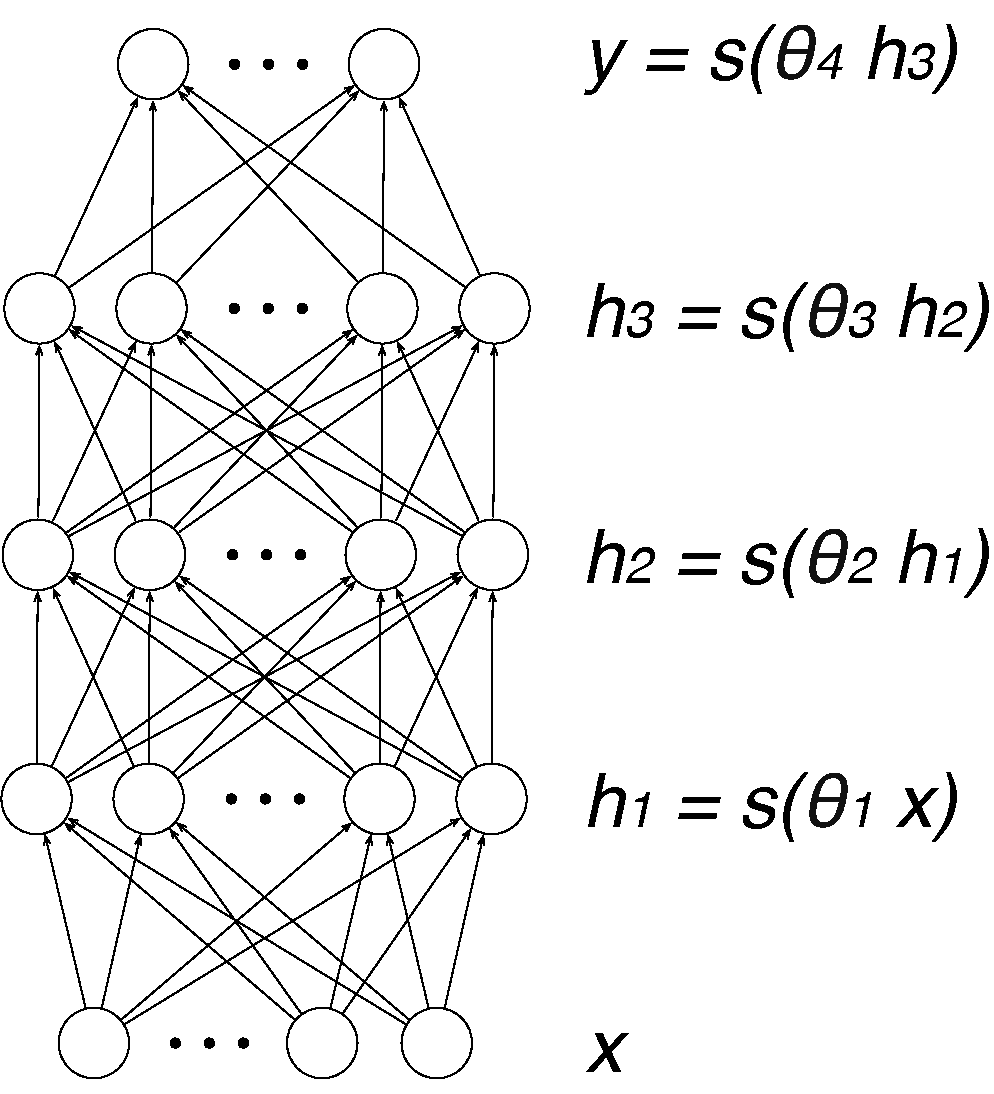
\includegraphics[scale=0.3]{nn3.pdf}
\end{frame}



\frame{\frametitle{history of neural networks 1}

\begin{description}
\item[1960s:] the linear perceptron learns from data (Rosenblatt et al)
\item[1969:] the perceptron can't do XOR (Minsky \& Papert)
\item[1970--1980:] nonlinear networks trained with back-propagation  (Linnainmaa; Dreyfus; Werbos; Rumelhart)
\item[1990s:] one hidden layer can represent any (Borel-measurable) function
\item[mid 90s:] NN's can't do everything / do not generalise / \dots
\item[mid 90s:] support vector machines (SVMs) are great!
\item[1995--2000:] SVM too slow / too many SVs
\end{description}
}



\begin{frame}
\frametitle{history of neural networks 2}

\begin{description}
\item[2000--:] probabilistic models for machine learning (ML)

\item[2006:] \textbf{deep neural networks}, trained with \textsl{Restricted Boltzmann Machines} and backprop

\item[2009:] deep NNs can be trained with just BP,  \textbf{much compute power} (GPU) and \textbf{enough data}

\item[2011--:] recurrent neural networks resurrect for time-series modelling

\item[2012--:] convolutional neural networks (CNN) start winning most vision benchmarks; recurrent neural networks applied to speech recognition in Android

\item[2013--:] \textbf{probabilistic} NN (variance propagation; variational autoencoder)

\item[2015--:] show cases in robotics, sensory processing, \dots

\item[2017:] ``Attention is all you need'' \dots
\end{description}
\end{frame}


\begin{frame}
\frametitle{a recurrent neural network has an internal state}
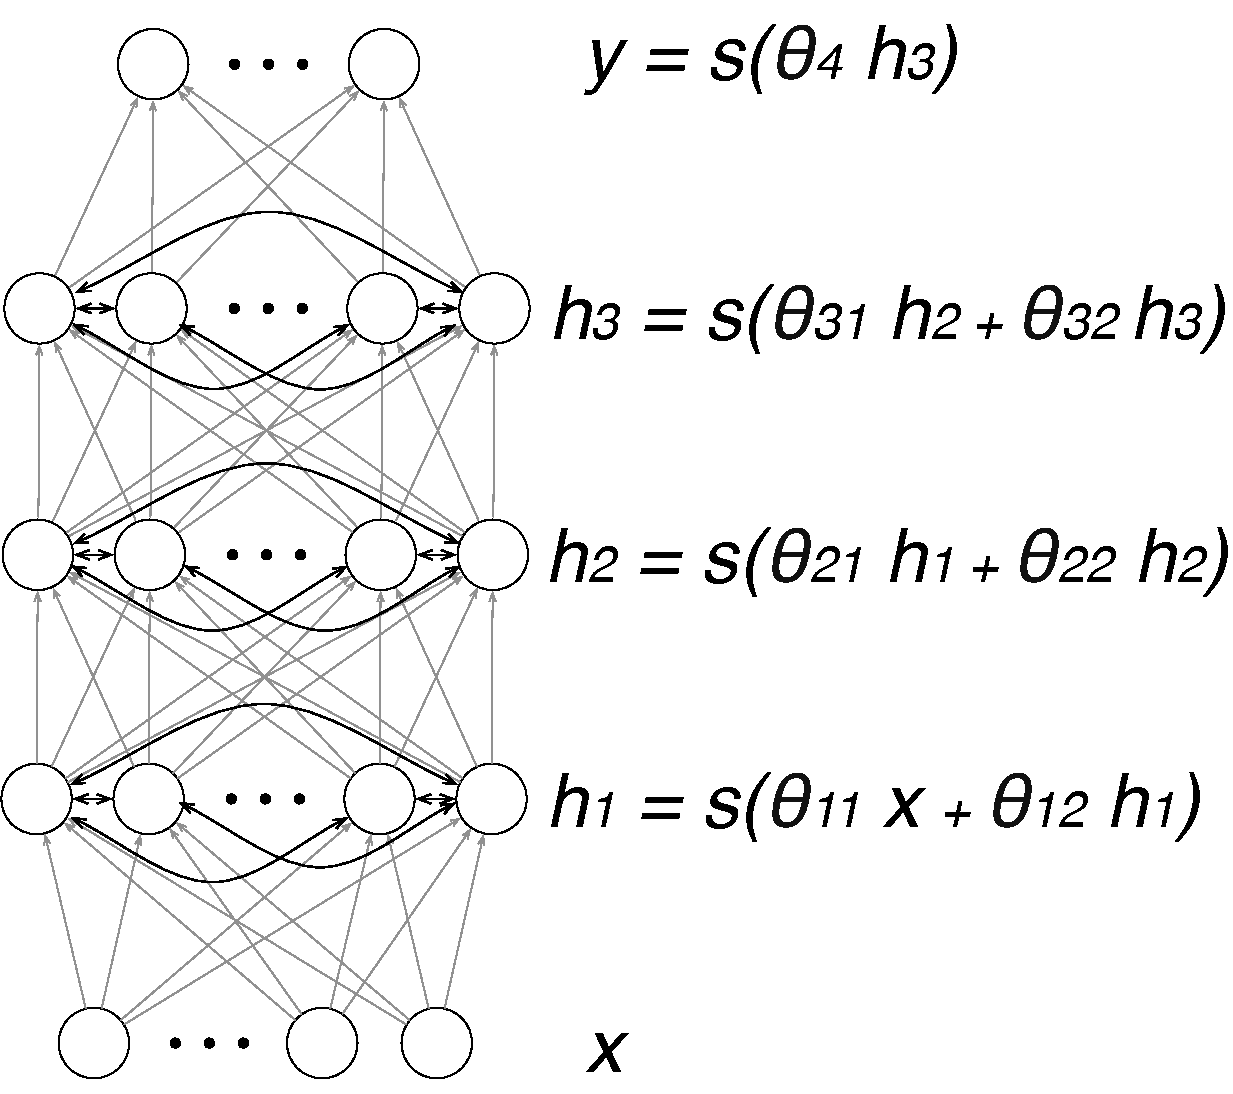
\includegraphics[scale=0.3]{nn4.pdf}
\end{frame}
\begin{frame}
\frametitle{autoencoder: NN in a special form}
 \begin{tikzpicture}[overlay]
   \node[shift={(9cm,-35mm)}](a) {Dim(latent space) $\ll$ Dim($x$)};
\end{tikzpicture}

\includegraphics[scale=0.3]{ae.pdf}
\end{frame}
\begin{frame}
\frametitle{VAE:  probabilistic AE}
\begin{tikzpicture}[overlay]
   \node[shift={(9cm,-35mm)}](a) {`nonlinear PCA'};
\end{tikzpicture}

\includegraphics[scale=0.3]{vae.pdf}
\end{frame}


%%%%%%%%%%%% Now to unsupervised vs supervised
%
%\begin{frame}
%\frametitle{supervised learning}
%given a data set ${\cal D} = \{(x_i, z_i)\}$ where $z_i = {\cal F}(x_i) + \epsilon_i$.  
%
%$x_i$ and $z_i$ are vectors.
%
%We cannot describe $\cal F$  mathematically.    How can we model $\cal F$?
%
%\bigskip\noindent
%\textsl{%
%Machine learning determines models (= parameterised models) \\to best approximate $\cal F$  by $\cal D$.}
%\end{frame}
%
%
%\begin{frame}
%\frametitle{supervised learning}
%\begin{columns}[t]
%\column{5cm}
%image recognition\\
%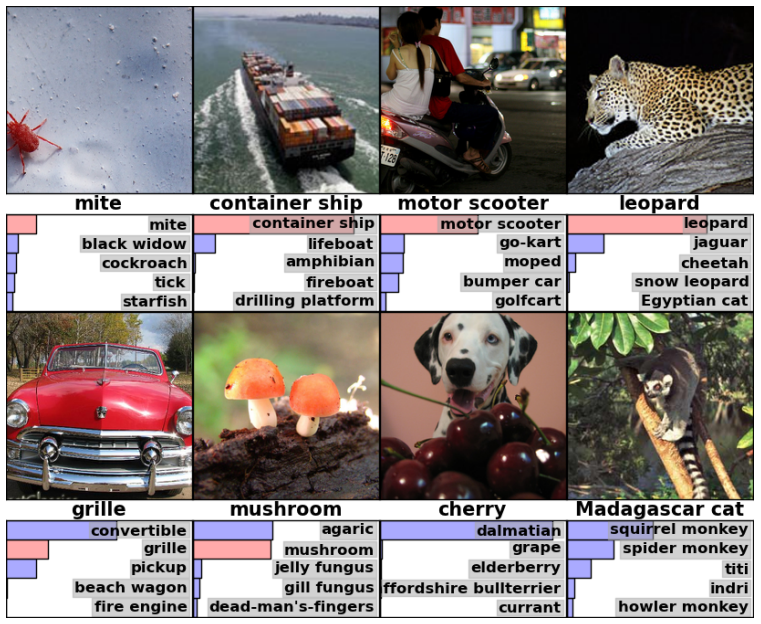
\includegraphics[width=\linewidth]{pics/objects}\\
%\vspace{.1cm}
%weather prediction\\
%\vspace{.1cm}
%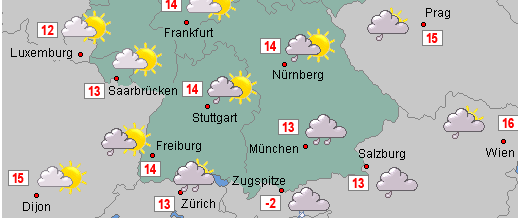
\includegraphics[width=\linewidth]{pics/weather}\\
%\column{5cm}
%stock prediction
%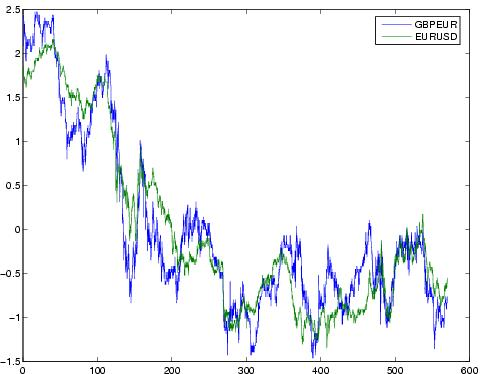
\includegraphics[width=\linewidth]{pics/financial}\\
%\vspace{.4cm}
%zip code recognition
%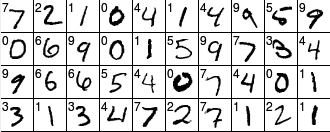
\includegraphics[width=\linewidth]{pics/mnist}\\
%\end{columns}
%
%\end{frame}
%
%
%
%
%
%\begin{frame}
%\frametitle{Un"uberwachtes Lernen (Engl: unsupervised learning)}
%
%given a data set ${\cal D} = \{(x_i)\}$ which is generated by a process $\cal F$.
%
%$x_i$ is a vector.
%
%We cannot describe $\cal F$  mathematically.    How can we model $\cal F$?
%
%\bigskip\noindent
%\textsl{%
%Machine learning determines models (= parameterised models) \\to best approximate $\cal F$  by $\cal D$.}
%
%\bigskip
%typical cases: \textsl{clustering}, \textsl{dimension reduction}
%\end{frame}
%
%
%
%
%
%\begin{frame}
%\frametitle{unsupervised learning}
%
%text analysis\\
%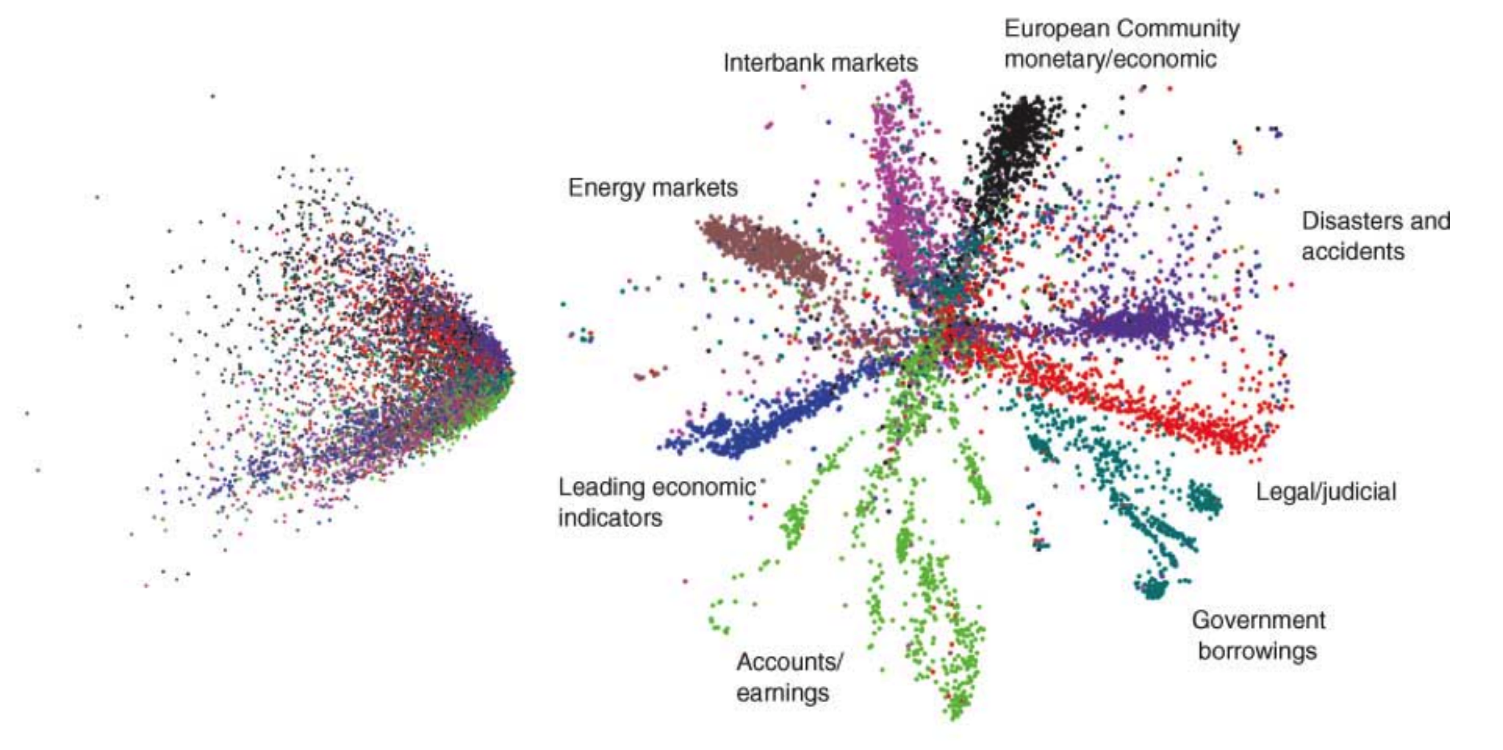
\includegraphics[width=10cm]{pics/autoencoder_nlp_exp.png}\\
%\vspace{1cm}
%\begin{columns}[t]
%\column{2cm}
%cocktail party
%\column{5cm}
%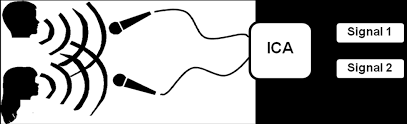
\includegraphics[width=5cm]{pics/ul-bss.png}
%\end{columns}
%\end{frame}



%
%\begin{frame}
%\frametitle{reinforcement learning}
%\begin{enumerate}
%\item 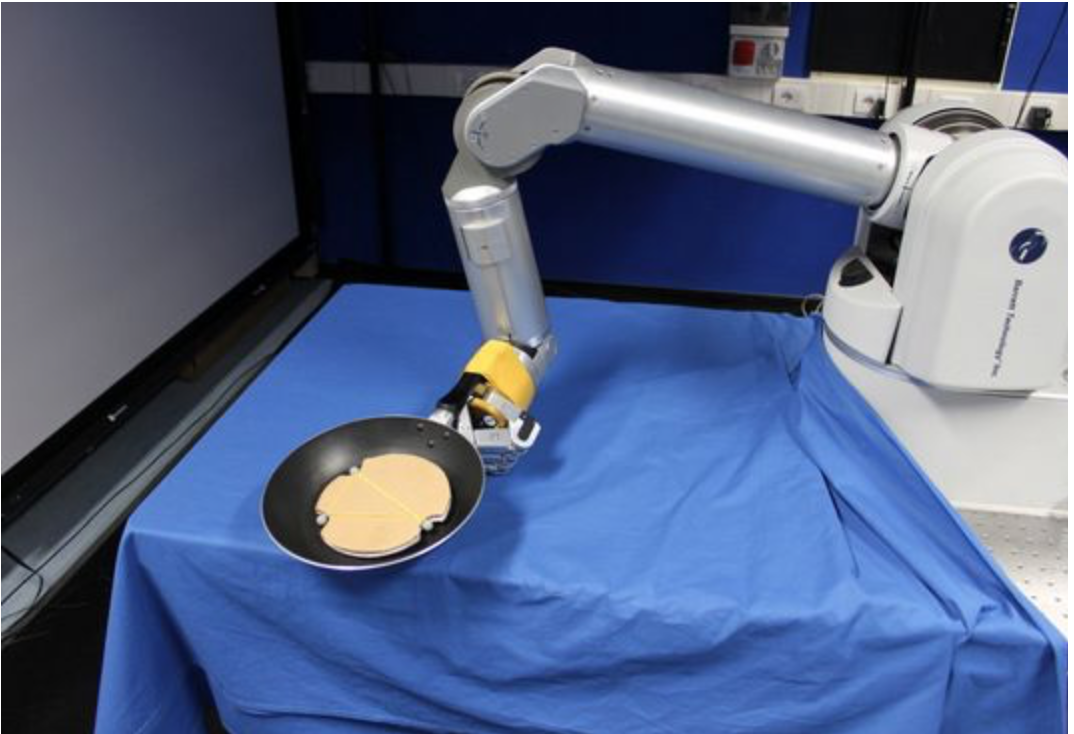
\includegraphics[width=6cm]{pancake}
%\item GM: PKW-Preisbestimmung
%\item Aufzugplanung
%\item Helikoptersteuerung
%\end{enumerate}
%\end{frame}
%
%
%
%
%
%\begin{frame}
%\frametitle{Best"arkendes Lernen (Engl: reinforcement learning)\\\small(auch: Verst"arkendes Lernen)}
%
%In einem System mit Zustand $s_i$ soll eine optimale Aktion $a_i$ gew"ahlt werden.
%
%Ziel: eine Strategie ("`policy"') finden um den zuk"unftigen Gewinn
%$$
%E[ r_t + \gamma r_{t+1} + \gamma^2 r_{t+2} + \dots ]  \quad \mathrm{mit\ } 0 \le \gamma \le 1
%$$
%zu maximieren.
%\end{frame}
%
%



%
%\begin{frame}
%\frametitle{learning and inference}
%
%if we have a model $${\cal M}(\theta): x\in\R^m \rightarrow y\in\R^n$$ und ein data set $${\cal D} = \{(x_i, z_i)\}$$
%then supervised learning means:
%$$
%\max_\theta p(y_i = z_i \mid x_i, \theta)
%$$
%
%\end{frame}




\begin{frame}
\frametitle{unsupervised learning: k-nearest neighbour}

 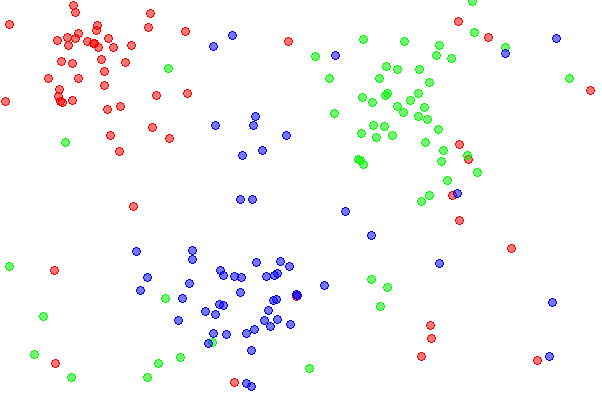
\includegraphics[width=\textwidth]{knn}

\end{frame}



\begin{frame}
\frametitle{1-NN algorithm}

Example: let's take $k=1$

\begin{enumerate}
\item define a distance measure
\item determine the number of classes
\item for each new data point $x$:
	\begin{enumerate}
	\item determine the distance to all other points
	\item find the nearest neighbours
	\end{enumerate}
\item the class $c$ of the new data point is determined
\end{enumerate}
\end{frame}



\begin{frame}
\frametitle{1-NN algorithm: overfitting}

 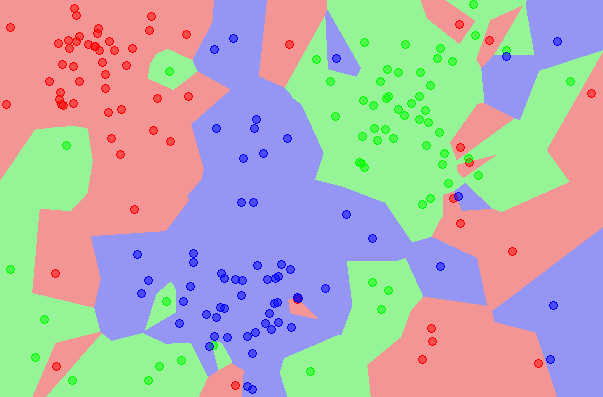
\includegraphics[width=\textwidth]{knn1}

\end{frame}



\begin{frame}
\frametitle{k-NN equation}

how can we describe this equation?

\pause

$$p(y = c \mid x) = {1 \over k} \sum_{i \in \mathrm{neighbours}} \delta_{y_ic}$$
mit
$$\delta_{ij} = \begin{cases}0 &\mathrm{if\ } i \neq j \\ 1 &\mathrm{if\ } i = j\end{cases}$$

\end{frame}



\begin{frame}
\frametitle{4-NN algorithm}

 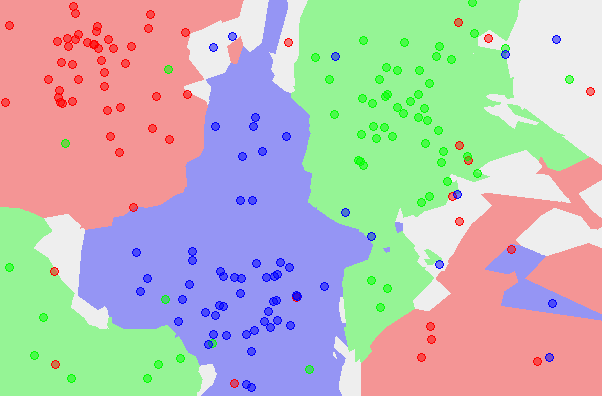
\includegraphics[width=\textwidth]{knn5}

\end{frame}



\begin{frame}
\frametitle{finding hyperparameters}

$k$ is a hyperparameter, the value of which determines the outcome.
How can we optimise it?

\bigskip
 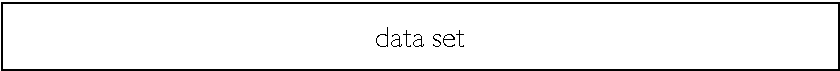
\includegraphics[scale=0.5]{xv0}

\pause
\bigskip
by cross validation

 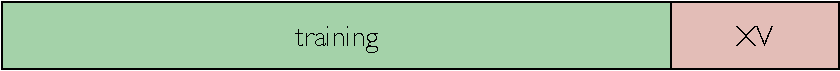
\includegraphics[scale=0.5]{xv1}

\end{frame}



 
\begin{frame}
\frametitle{finding hyperparameters}
5-fold crossvalidation

 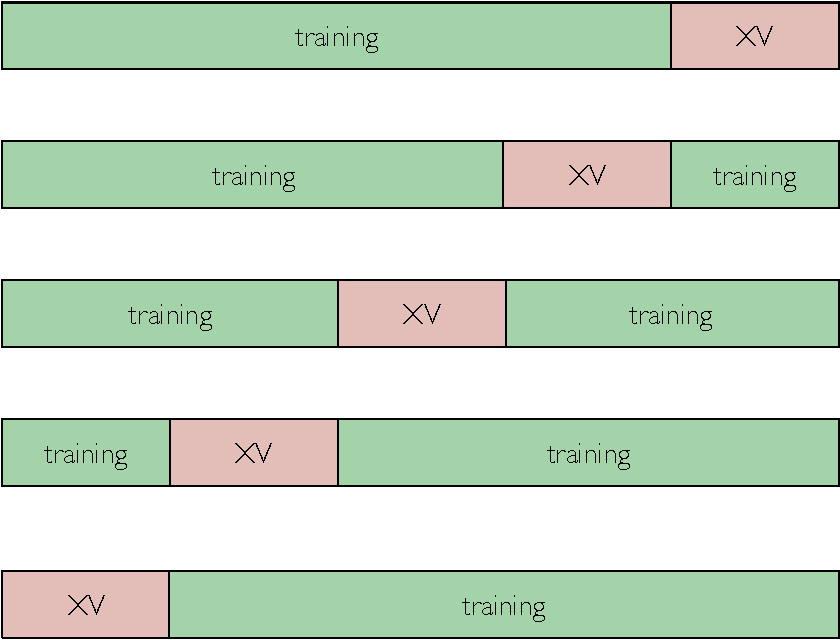
\includegraphics[scale=0.5]{xv2}

\end{frame}


\begin{frame}
\frametitle{finding hyperparameters}
but a more honest method is:
\begin{enumerate}
\item first learn\\
 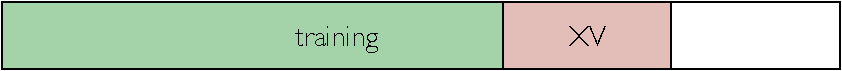
\includegraphics[scale=0.5]{xv3}
 \bigskip
\item \pause then test on new data\\
 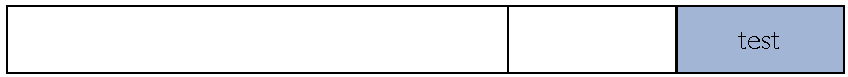
\includegraphics[scale=0.5]{xv4}
\end{enumerate}

\end{frame}



\begin{frame}
\frametitle{problems with kNN}

\begin{itemize}
\item finding the right distance measure is difficult and strongly influences the result
\item in high-dimensional spaces, distances stop making sense
{\tiny \url{https://stats.stackexchange.com/questions/99171/why-is-euclidean-distance-not-a-good-metric-in-high-dimensions}}
\item finding the neighbours is very  expensive in high-dimensional spaces
\item finding the neighbours is  very expensive if many data exist
\end{itemize}
\end{frame}


\end{document}
